\documentclass{ximera}

\author{Anna Davis \and Rosemarie Emanuele} \title{Introduction to Linear Combinations and Span of Vectors} \license{CC-BY 4.0}

\renewcommand{\vec}[1]{{\bf #1}}
\newcommand{\RR}{\mathbb{R}}
\newcommand{\dfn}{\textit}
\newcommand{\dotp}{\cdot}
\newcommand{\id}{\text{id}}

\newtheorem{general}{Generalization}
\newtheorem{initprob}{Exploration Problem}
\usepackage{tikz-cd}
\usepackage{tikz-3dplot}
\usetikzlibrary{shapes.geometric}
\usetikzlibrary{arrows}
\pgfplotsset{compat=1.14}



\begin{document}
\begin{abstract}
  We define a linear combination of vectors, the span of a set of vectors, and examine linear combinations and span using geometric intuition.
\end{abstract}
\maketitle

\section*{Linear Combinations of Vectors}

\begin{definition}
A vector $\vec{v}$ is said to be a linear combination of vectors $\vec{v}_1, \vec{v}_2,\ldots, \vec{v}_n$ if 
$$\vec{v}=a_1\vec{v}_1+ a_2\vec{v}_2+\ldots + a_n\vec{v}_n$$
for some scalars $a_1, a_2, \ldots ,a_n$.
\end{definition}
For example, $\begin{bmatrix} -4\\9\\-10\\-1\end{bmatrix}$ is a linear combination of $\begin{bmatrix} -1\\3\\-3\\0\end{bmatrix}$,
$\begin{bmatrix} 2\\0\\1\\4\end{bmatrix}$ and $\begin{bmatrix} 0\\1\\-1\\1\end{bmatrix}$ because 
$$\begin{bmatrix} -4\\9\\-10\\-1\end{bmatrix}=2\begin{bmatrix} -1\\3\\-3\\0\end{bmatrix}+(-1)\begin{bmatrix} 2\\0\\1\\4\end{bmatrix}+3\begin{bmatrix} 0\\1\\-1\\1\end{bmatrix}$$

In this module we will focus on vectors in $\RR^2$ and $\RR^3$.
\subsection*{Geometry of Linear Combinations}

\begin{example}
Express $\begin{bmatrix}2\\4\end{bmatrix}$ as a linear combination of $\begin{bmatrix}2\\1\end{bmatrix}$ and $\begin{bmatrix}2\\-2\end{bmatrix}$.  Interpret your results geometrically.
\begin{explanation}
We need to find scalars $a$ and $b$ such that 
$$\begin{bmatrix}2\\4\end{bmatrix}=a\begin{bmatrix}2\\1\end{bmatrix}+b\begin{bmatrix}2\\-2\end{bmatrix}$$
This amounts to solving a system of linear equations
\begin{align*}
2a+2b&=2\\
a-2b&=4
\end{align*}
Use your favorite method to solve this system.  You will find that $a=2$ and $b=-1$.  Now we can write $\begin{bmatrix}2\\4\end{bmatrix}$ as a linear combination of $\begin{bmatrix}2\\1\end{bmatrix}$ and $\begin{bmatrix}2\\-2\end{bmatrix}$ as follows:

$$\begin{bmatrix}2\\4\end{bmatrix}=2\begin{bmatrix}2\\1\end{bmatrix}+(-1)\begin{bmatrix}2\\-2\end{bmatrix}$$

Geometrically speaking, this means that the vector $\begin{bmatrix}2\\4\end{bmatrix}$ is the diagonal of the parallelogram determined by $2\begin{bmatrix}2\\1\end{bmatrix}$ and $(-1)\begin{bmatrix}2\\-2\end{bmatrix}$.  The original vectors $\begin{bmatrix}2\\1\end{bmatrix}$ and $\begin{bmatrix}2\\-2\end{bmatrix}$ are shown below together with the parallelogram and its diagonal. 

\begin{image}[3.5in]
\begin{tikzpicture}[scale=1]
\draw[thin,gray!40] (-4,-4) grid (4,4);
  \draw[<->] (-4,0)--(4,0);
  \draw[<->] (0,-4)--(0,4);
  
  \filldraw[blue, opacity=0.3](0,0)--(-2,2)--(2,4)--(4,2)--cycle;
\draw[line width=2pt,red,-stealth](0,0)--(2,1) node[below right]{$\begin{bmatrix}2\\1\end{bmatrix}$};
\draw[line width=2pt,red,-stealth, dashed](0,0)--(4,2) node[below right]{$2\begin{bmatrix}2\\1\end{bmatrix}$};
 % \fill[blue!40!white] (10,0) circle (0.2cm);
 \draw[line width=2pt,blue,-stealth](0,0)--(2,-2) node[right]{$\begin{bmatrix}2\\-2\end{bmatrix}$};
 \draw[line width=2pt,blue,-stealth, dashed](0,0)--(-2,2) node[above left]{$(-1)\begin{bmatrix}2\\-2\end{bmatrix}$};
 \draw[line width=2pt,-stealth](0,0)--(2,4); 
\end{tikzpicture}
\end{image}

\end{explanation}
\end{example}

\begin{example}\label{ex:lincombparallelogrammethod}
Use geometry to express $\begin{bmatrix}3\\-4\end{bmatrix}$ as a linear combination of $\begin{bmatrix}-1\\3\end{bmatrix}$ and $\begin{bmatrix}-4\\2\end{bmatrix}$.
\begin{explanation}
We are looking for $\begin{bmatrix}3\\-4\end{bmatrix}$ to be the diagonal of a parallelogram determined by scalar multiples of $\begin{bmatrix}-1\\3\end{bmatrix}$ and $\begin{bmatrix}-4\\2\end{bmatrix}$.  

\begin{image}
\begin{tikzpicture}[scale=0.8]
\draw[thin,gray!40] (-4,-4) grid (4,4);
  \draw[<->] (-4,0)--(4,0);
  \draw[<->] (0,-4)--(0,4);
  
\draw[line width=2pt,red,-stealth](0,0)--(-1,3) node[left]{$\begin{bmatrix}-1\\3\end{bmatrix}$};

 \draw[line width=2pt,blue,-stealth](0,0)--(-4,2) node[above right]{$\begin{bmatrix}-4\\2\end{bmatrix}$};

 \draw[line width=2pt,-stealth](0,0)--(3,-4)node[right]{$\begin{bmatrix}3\\-4\end{bmatrix}$}; 

\end{tikzpicture}
\end{image}

Because a scalar multiple of a vector can point in the same direction as the vector or in the opposite direction, we will start by drawing straight lines determined by the two vectors.

\begin{image}
\begin{tikzpicture}[scale=0.8]
\draw[thin,gray!40] (-4,-4) grid (4,4);
  \draw[<->] (-4,0)--(4,0);
  \draw[<->] (0,-4)--(0,4);
  

\draw[line width=2pt,red,-stealth](0,0)--(-1,3) node[left]{$\begin{bmatrix}-1\\3\end{bmatrix}$};
\draw[line width=1pt,red, dashed](4/3,-4)--(-4/3,4) ;


 \draw[line width=2pt,blue,-stealth](0,0)--(-4,2) node[above right]{$\begin{bmatrix}-4\\2\end{bmatrix}$};
\draw[line width=1pt,blue, dashed](-4,2)--(4,-2) ;
 
 \draw[line width=2pt,-stealth](0,0)--(3,-4)node[right]{$\begin{bmatrix}3\\-4\end{bmatrix}$}; 
 
\end{tikzpicture}
\end{image}

The two lines that we drew will contain the sides of the parallelogram we are looking for.  To find the other two sides we will draw lines parallel to $\begin{bmatrix}-1\\3\end{bmatrix}$ and $\begin{bmatrix}-4\\2\end{bmatrix}$ through the head of vector $\begin{bmatrix}3\\-4\end{bmatrix}$.

\begin{image}
\begin{tikzpicture}[scale=0.8]
\draw[thin,gray!40] (-4,-4) grid (4,4);
  \draw[<->] (-4,0)--(4,0);
  \draw[<->] (0,-4)--(0,4);
  
\draw[line width=2pt,red,-stealth](0,0)--(-1,3) node[left]{$\begin{bmatrix}-1\\3\end{bmatrix}$};
\draw[line width=1pt,red, dashed](4/3,-4)--(-4/3,4) ;
\draw[line width=1pt,red, dashed](3,-4)--(1/3,4) ;

 \draw[line width=2pt,blue,-stealth](0,0)--(-4,2) node[above right]{$\begin{bmatrix}-4\\2\end{bmatrix}$};
\draw[line width=1pt,blue, dashed](-4,2)--(4,-2) ;
  \draw[line width=1pt,blue, dashed](-4,-0.5)--(3,-4) ;
 \draw[line width=2pt,-stealth](0,0)--(3,-4)node[right]{$\begin{bmatrix}3\\-4\end{bmatrix}$}; 
 
\end{tikzpicture}
\end{image}

Now the parallelogram is clearly visible.

\begin{image}
\begin{tikzpicture}[scale=0.8]
\draw[thin,gray!40] (-4,-4) grid (4,4);
  \draw[<->] (-4,0)--(4,0);
  \draw[<->] (0,-4)--(0,4);
  
 \filldraw[blue, opacity=0.3](0,0)--(1,-3)--(3,-4)--(2,-1)--cycle;
\draw[line width=2pt,red,-stealth](0,0)--(-1,3) node[left]{$\begin{bmatrix}-1\\3\end{bmatrix}$};
\draw[line width=1pt,red, dashed](4/3,-4)--(-4/3,4) ;
\draw[line width=1pt,red, dashed](3,-4)--(1/3,4) ;

 \draw[line width=2pt,blue,-stealth](0,0)--(-4,2) node[above right]{$\begin{bmatrix}-4\\2\end{bmatrix}$};
\draw[line width=1pt,blue, dashed](-4,2)--(4,-2) ;
  \draw[line width=1pt,blue, dashed](-4,-0.5)--(3,-4) ;
 \draw[line width=2pt,-stealth](0,0)--(3,-4)node[right]{$\begin{bmatrix}3\\-4\end{bmatrix}$}; 
 
\end{tikzpicture}
\end{image}

The last remaining task is to identify the sides of the parallelogram as scalar multiples of $\begin{bmatrix}-1\\3\end{bmatrix}$ and $\begin{bmatrix}-4\\2\end{bmatrix}$.  We do this by identifying vectors $\begin{bmatrix}1\\-3\end{bmatrix}$ and $\begin{bmatrix}2\\-1\end{bmatrix}$ as the vectors that determine the parallelogram.

\begin{image}
\begin{tikzpicture}[scale=0.8]
\draw[thin,gray!40] (-4,-4) grid (4,4);
  \draw[<->] (-4,0)--(4,0);
  \draw[<->] (0,-4)--(0,4);
  
 \filldraw[blue, opacity=0.3](0,0)--(1,-3)--(3,-4)--(2,-1)--cycle;
\draw[line width=2pt,red,-stealth](0,0)--(-1,3) node[left]{$\begin{bmatrix}-1\\3\end{bmatrix}$};
\draw[line width=1pt,red, dashed](4/3,-4)--(-4/3,4) ;
\draw[line width=1pt,red, dashed](3,-4)--(1/3,4) ;

 \draw[line width=2pt,blue,-stealth](0,0)--(-4,2) node[above right]{$\begin{bmatrix}-4\\2\end{bmatrix}$};
\draw[line width=1pt,blue, dashed](-4,2)--(4,-2) ;
  \draw[line width=1pt,blue, dashed](-4,-0.5)--(3,-4) ;
 \draw[line width=2pt,-stealth](0,0)--(3,-4)node[right]{$\begin{bmatrix}3\\-4\end{bmatrix}$}; 
 
  \fill[red] (1,-3) node[below left]{$(1,-3)$} circle (0.1cm);
  \fill[blue] (2,-1) node[above right]{$(2,-1)$} circle (0.1cm);
\end{tikzpicture}
\end{image}

Observe that vector $\begin{bmatrix}2\\-1\end{bmatrix}$ is half the length of $\begin{bmatrix}-4\\2\end{bmatrix}$ and points in the opposite direction, while the vector $\begin{bmatrix}1\\-3\end{bmatrix}$ is the same length as $\begin{bmatrix}-1\\3\end{bmatrix}$ and also points in the opposite direction.

Now we can write $\begin{bmatrix}3\\-4\end{bmatrix}$ as a linear combination of $\begin{bmatrix}-1\\3\end{bmatrix}$ and $\begin{bmatrix}-4\\2\end{bmatrix}$ as follows
 $$\begin{bmatrix}3\\-4\end{bmatrix}=\begin{bmatrix}1\\-3\end{bmatrix}+\begin{bmatrix}2\\-1\end{bmatrix}=(-1)\begin{bmatrix}-1\\3\end{bmatrix}+\left(-\frac{1}{2}\right)\begin{bmatrix}-4\\2\end{bmatrix}$$
\end{explanation}
\end{example}

The method we used in Example \ref{ex:lincombparallelogrammethod} to express the given vector as a linear combination of two other vectors is sufficiently useful that we summarize the steps.

\begin{procedure}\label{pro:lincombgeo} Given two non-collinear vectors $\vec{u}$ and $\vec{v}$ in $\RR^2$, and a vector $\vec{w}$ which is not a scalar multiple of either $\vec{u}$ or $\vec{v}$, we can express $\vec{w}$ as a linear combination of $\vec{u}$ and $\vec{v}$ as follows:
\begin{enumerate}
\item Draw lines $L_{\vec{u}}$ and $L_{\vec{v}}$ determined by $\vec{u}$ and $\vec{v}$, respectively.
\item Through the head of vector $\vec{w}$, draw lines $P_{\vec{u}}$ and $P_{\vec{v}}$, parallel to $L_{\vec{u}}$ and $L_{\vec{v}}$, respectively.
\item Let $A$ be the point of intersection of $P_{\vec{u}}$ and $L_{\vec{v}}$.
\item Let $B$ be the point of intersection of $P_{\vec{v}}$ and $L_{\vec{u}}$.
\item Let $O$ denote the origin.  Then $\overrightarrow{OA}=k_1\vec{v}$ and $\overrightarrow{OB}=k_2\vec{u}$ for some scalars $k_1$ and $k_2$.  
\item We have $\vec{w}=k_2\vec{u}+k_1\vec{v}$.
\end{enumerate}

\begin{image}
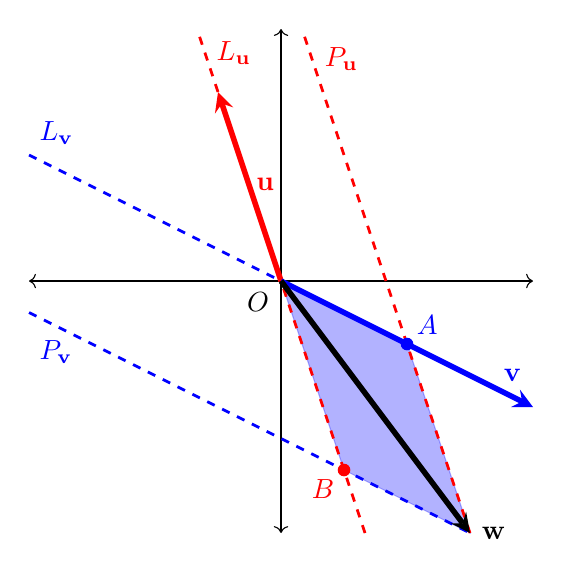
\begin{tikzpicture}[scale=0.8]

  \draw[<->] (-4,0)--(4,0);
  \draw[<->] (0,-4)--(0,4);
  
 \filldraw[blue, opacity=0.3](0,0)--(1,-3)--(3,-4)--(2,-1)--cycle;
\draw[line width=2pt,red,-stealth](0,0)node[right=-2mm,above=10mm]{$\vec{u}$}--(-1,3) node[right=2mm,above=2mm]{$L_{\vec{u}}$};
\draw[line width=1pt,red, dashed](4/3,-4)--(-4/3,4) ;
\draw[line width=1pt,red, dashed](3,-4)--(1/3,4)node[right=5mm, below=1mm]{$P_{\vec{u}}$} ;

 \draw[line width=2pt,blue,-stealth](0,0)--(4,-2) node[above=4mm, left=0mm]{$\vec{v}$};
\draw[line width=1pt,blue, dashed](-4,2)node[above right]{$L_{\vec{v}}$}--(4,-2) ;
  \draw[line width=1pt,blue, dashed](-4,-0.5)node[below=5mm, right]{$P_{\vec{v}}$}--(3,-4) ;
 \draw[line width=2pt,-stealth](0,0)node[below left]{$O$}--(3,-4)node[right]{$\vec{w}$}; 
 
  \fill[red] (1,-3) node[below left]{$B$} circle (0.1cm);
  \fill[blue] (2,-1) node[above right]{$A$} circle (0.1cm);
\end{tikzpicture}
\end{image}
\end{procedure}

\begin{example}
Can the vector $\begin{bmatrix}1\\4\end{bmatrix}$ be written as a linear combination of vectors $\begin{bmatrix}-3\\1\end{bmatrix}$ and $\begin{bmatrix}6\\-2\end{bmatrix}$?
\begin{explanation}
We will start with a geometric approach.
\begin{image}
\begin{tikzpicture}[scale=0.8]
\draw[thin,gray!40] (-4,-5) grid (7,4);
  \draw[<->] (-4,0)--(7,0);
  \draw[<->] (0,-5)--(0,4);
  
 
\draw[line width=2pt,red,-stealth](0,0)--(-3,1) node[above right]{$\begin{bmatrix}-3\\1\end{bmatrix}$};

 \draw[line width=2pt,blue,-stealth](0,0)--(6,-2) node[below left]{$\begin{bmatrix}6\\-2\end{bmatrix}$};

 \draw[line width=2pt,-stealth](0,0)--(3,2)node[right]{$\begin{bmatrix}3\\2\end{bmatrix}$}; 
 
\end{tikzpicture}
\end{image}

Observe that $\begin{bmatrix}-3\\1\end{bmatrix}$ and $\begin{bmatrix}6\\-2\end{bmatrix}$ are scalar multiples of each other and lie on the same line.  

A linear combination of $\begin{bmatrix}-3\\1\end{bmatrix}$ and $\begin{bmatrix}6\\-2\end{bmatrix}$ has the form:

$$a\begin{bmatrix}6\\-2\end{bmatrix}+b\begin{bmatrix}-3\\1\end{bmatrix}=a(-2)\begin{bmatrix}-3\\1\end{bmatrix}+b\begin{bmatrix}-3\\1\end{bmatrix}=(-2a+b)\begin{bmatrix}-3\\1\end{bmatrix}$$

This shows that all linear combinations of $\begin{bmatrix}-3\\1\end{bmatrix}$ and $\begin{bmatrix}6\\-2\end{bmatrix}$ will be scalar multiples of $\begin{bmatrix}-3\\1\end{bmatrix}$, and therefore lie on the same line as $\begin{bmatrix}-3\\1\end{bmatrix}$.
Since $\begin{bmatrix}3\\2\end{bmatrix}$ does not lie on the line determined by $\begin{bmatrix}-3\\1\end{bmatrix}$ it cannot be expressed as a linear combination of $\begin{bmatrix}-3\\1\end{bmatrix}$ and $\begin{bmatrix}6\\-2\end{bmatrix}$.

We can also address this question algebraically.  To express $\begin{bmatrix}3\\2\end{bmatrix}$ as a linear combination of $\begin{bmatrix}-3\\1\end{bmatrix}$ and $\begin{bmatrix}6\\-2\end{bmatrix}$, we need to solve the equation.
$$a\begin{bmatrix}-3\\1\end{bmatrix}+b\begin{bmatrix}6\\-2\end{bmatrix}=\begin{bmatrix}3\\2\end{bmatrix}$$
This gives us a system of equations
\begin{align*}
-3a+6b&=3\\
a-2b&=2
\end{align*}

When you try to solve this system using your favorite method, you will find that the system is inconsistent.  Thus, $\begin{bmatrix}3\\2\end{bmatrix}$ cannot be written as a linear combination of $\begin{bmatrix}-3\\1\end{bmatrix}$ and $\begin{bmatrix}6\\-2\end{bmatrix}$.

\end{explanation}
\end{example}

\subsection*{Algebra of Linear Combinations}

\begin{example}
If possible, express $\begin{bmatrix}7\\4\\-5\end{bmatrix}$ as a linear combination of $\begin{bmatrix}1\\-2\\1\end{bmatrix}$ and $\begin{bmatrix}3\\0\\-1\end{bmatrix}$.
\begin{explanation}
We are looking for coefficients $a$ and $b$ such that 
$$a\begin{bmatrix}1\\-2\\1\end{bmatrix}+b\begin{bmatrix}3\\0\\-1\end{bmatrix}=\begin{bmatrix}7\\4\\-5\end{bmatrix}$$
This translates into a system of equations
\begin{align*}
a+3b&=7\\
-2a&=4\\
a-b&=-5
\end{align*}
Solve this system for $a$ and $b$, and enter your answers below:
$$a=\answer{-2}\quad\text{and}\quad b=\answer{3}$$
We conclude that $\begin{bmatrix}7\\4\\-5\end{bmatrix}$ is a linear combination of $\begin{bmatrix}1\\-2\\1\end{bmatrix}$ and $\begin{bmatrix}3\\0\\-1\end{bmatrix}$, and write:
$$\begin{bmatrix}7\\4\\-5\end{bmatrix}=\answer{-2}\begin{bmatrix}1\\-2\\1\end{bmatrix}+\answer{3}\begin{bmatrix}3\\0\\-1\end{bmatrix}$$
\end{explanation}
\end{example}

\begin{example}
Set up a system of equations that can be used to express $\begin{bmatrix}2\\-1\\3\\0\end{bmatrix}$ as a linear combination of $\begin{bmatrix}1\\0\\4\\-2\end{bmatrix}$, $\begin{bmatrix}-2\\-1\\1\\-1\end{bmatrix}$, $\begin{bmatrix}0\\4\\-3\\1\end{bmatrix}$ and $\begin{bmatrix}1\\1\\-1\\4\end{bmatrix}$, or to determine that such a combination does not exist.  Do not solve the system.
\begin{explanation}
We are looking for $x_1$, $x_2$, $x_3$ and $x_4$ such that 
$$x_1\begin{bmatrix}1\\0\\4\\-2\end{bmatrix}+x_2\begin{bmatrix}-2\\-1\\1\\-1\end{bmatrix}+x_3\begin{bmatrix}0\\4\\-3\\1\end{bmatrix}+x_4\begin{bmatrix}1\\1\\-1\\4\end{bmatrix}=\begin{bmatrix}2\\-1\\3\\0\end{bmatrix}$$
This translates into the following system of equations:

$$\begin{array}{ccccccccc}
      x_1 & -&2x_2 & & &+ & x_4&= &2 \\
        & &-x_2  &+ &4x_3 & +& x_4&= &-1 \\
      4x_1 &+ &x_2 & -&3x_3 &-&x_4&= &3\\
	 -2x_1& -&x_2 & +&x_3&+&4x_4&=&0
    \end{array}$$
    At this point you may not have the techniques for solving this system of equations efficiently.  So, we present this problem as an example of a set-up only.  Later in the course you will learn to solve and interpret such systems.
\end{explanation}
\end{example}

\section*{Span}
In the previous section we considered different ways for determining whether one given vector is a linear combination of a collection of vectors.  In this section, we consider the set of all linear combinations of a collection of vectors.
\begin{definition}\label{def:span} Let $\vec{v}_1, \vec{v}_2,\ldots ,\vec{v}_m$ be vectors in $\RR^n$.  The set $S$ of all linear combinations of $\vec{v}_1, \vec{v}_2,\ldots ,\vec{v}_m$ is called the span of $\vec{v}_1, \vec{v}_2,\ldots ,\vec{v}_m$.  We write 
$$S=\textnormal{span}(\vec{v}_1, \vec{v}_2,\ldots ,\vec{v}_m)$$
and we say that $\vec{v}_1, \vec{v}_2,\ldots ,\vec{v}_m$ span $S$.
\end{definition}

\begin{example}
Describe $\textnormal{span}\left(\begin{bmatrix}-3\\1\end{bmatrix}\right)$.
\begin{explanation}
The span of $\begin{bmatrix}-3\\1\end{bmatrix}$ is the set of all linear combinations of $\begin{bmatrix}-3\\1\end{bmatrix}$.  Since we are looking for linear combinations of only one vector, we are really looking for all of its scalar multiples.  So, the span will be the set of all vectors of the form $\vec{v}=a\begin{bmatrix}-3\\1\end{bmatrix}$.  All such vectors lie on the line determined by $\begin{bmatrix}-3\\1\end{bmatrix}$.

\begin{image}[3.5in]
\begin{tikzpicture}[scale=0.8]
\draw[thin,gray!40] (-6,-4) grid (6,4);
  \draw[<->] (-6,0)--(6,0);
  \draw[<->] (0,-4)--(0,4);
  
 \draw[line width=1pt,-stealth](0,0)--(-6,2);
 \draw[line width=1pt,-stealth](0,0)--(6,-2);
 \draw[line width=1pt,-stealth](0,0)--(3,-1);
 \draw[line width=1pt,-stealth](0,0)--(1.5,-0.5);
 \draw[line width=1pt,-stealth](0,0)--(4.5,-1.5);
 \draw[line width=1pt,-stealth](0,0)--(-4.5,1.5);

 \draw[line width=2pt,red,-stealth](0,0)--(-3,1) node[above right]{$\begin{bmatrix}-3\\1\end{bmatrix}$};

 \end{tikzpicture}
\end{image}


\end{explanation}
\end{example}

\begin{example}
Describe $\textnormal{span}\left(\begin{bmatrix}2\\2\end{bmatrix}, \begin{bmatrix}-1\\0\end{bmatrix}\right)$.
\begin{explanation}
First, observe that $\begin{bmatrix}2\\2\end{bmatrix}$ and $\begin{bmatrix}-1\\0\end{bmatrix}$ are not scalar multiples of each other, so they do not lie on the same line.  

\begin{image}[3in]
\begin{tikzpicture}[scale=0.8]
\draw[thin,gray!40] (-4,-1) grid (4,4);
  \draw[<->] (-4,0)--(4,0);
  \draw[<->] (0,-1)--(0,4);
  
  \draw[line width=2pt,blue,-stealth](0,0)--(2,2) node[above right]{$\begin{bmatrix}2\\2\end{bmatrix}$};
  \draw[line width=2pt,red,-stealth](0,0)--(-1,0) node[above left]{$\begin{bmatrix}-1\\0\end{bmatrix}$};

 \end{tikzpicture}
\end{image}


If $\vec{w}$ is a scalar multiple of one of $\begin{bmatrix}2\\2\end{bmatrix}, \begin{bmatrix}-1\\0\end{bmatrix}$, then $\vec{w}$ is in $\textnormal{span}\left(\begin{bmatrix}2\\2\end{bmatrix}, \begin{bmatrix}-1\\0\end{bmatrix}\right)$.  Otherwise, we can use Procedure \ref{pro:lincombgeo} to express $\vec{w}$ as a linear combination of $\begin{bmatrix}2\\2\end{bmatrix}, \begin{bmatrix}-1\\0\end{bmatrix}$.  This shows that every vector of $\RR^2$ can be written as a linear combination of $\begin{bmatrix}2\\2\end{bmatrix}, \begin{bmatrix}-1\\0\end{bmatrix}$. We conclude that $\textnormal{span}\left(\begin{bmatrix}2\\2\end{bmatrix}, \begin{bmatrix}-1\\0\end{bmatrix}\right)=\RR^2$.
\end{explanation}
\end{example}

\begin{example}\label{ex:spanoftwovectors}
Describe $\textnormal{span}\left(\begin{bmatrix}5\\0\\4\end{bmatrix}, \begin{bmatrix}0\\4\\2\end{bmatrix}\right)$.
\begin{explanation}
First, observe that $\begin{bmatrix}5\\0\\4\end{bmatrix}, \begin{bmatrix}0\\4\\2\end{bmatrix}$ are not scalar multiples of each other, so they do not lie on the same line.  

\begin{image}
\tdplotsetmaincoords{70}{130}
\begin{tikzpicture}
	\draw[->](-2,0,0)--(5,0,0) node[below left]{$y$};
    \draw[->](0,-2,0)--(0,5,0) node[below left]{$z$};
    \draw[->](0,0,-2)--(0,0,5) node[below left]{$x$};
    
    \draw[->, line width=2pt,blue, -stealth](0,0,0)--(0,4,5)node[above right]{$\begin{bmatrix}5\\0\\4\end{bmatrix}$};
    \draw[->, line width=2pt,red, -stealth](0,0,0)--(4,2,0)node[above left]{$\begin{bmatrix}0\\4\\2\end{bmatrix}$};
    
\end{tikzpicture}
\end{image}

The span of $\begin{bmatrix}5\\0\\4\end{bmatrix}$ and $\begin{bmatrix}0\\4\\2\end{bmatrix}$ consists of elements of the form
$$a\begin{bmatrix}5\\0\\4\end{bmatrix}+b\begin{bmatrix}0\\4\\2\end{bmatrix}$$

Geometrically, we can interpret all such linear combinations as diagonals of parallelograms determined by scalar multiples of $\begin{bmatrix}5\\0\\4\end{bmatrix}$ and $\begin{bmatrix}0\\4\\2\end{bmatrix}$.  All such diagonals will lie in the same plane.  Let this plane be called $p$.  A portion of $p$ is shown below.
\begin{image}
\tdplotsetmaincoords{70}{130}
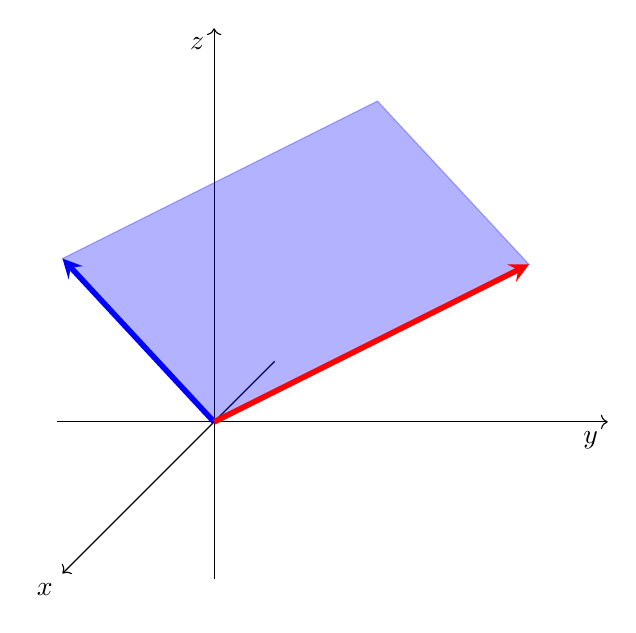
\begin{tikzpicture}
	\draw[->](-2,0,0)--(5,0,0) node[below left]{$y$};
    \draw[->](0,-2,0)--(0,5,0) node[below left]{$z$};
    \draw[->](0,0,-2)--(0,0,5) node[below left]{$x$};
    \filldraw[blue, opacity=0.3] (0,0,0)--(4, 2, 0)--(4,6,5)--(0, 4, 5)--cycle;
    \draw[->, line width=2pt,blue, -stealth](0,0,0)--(0,4,5);
    \draw[->, line width=2pt,red, -stealth](0,0,0)--(4,2,0);
    
\end{tikzpicture}
\end{image}

Because Procedure \ref{pro:lincombgeo} can be applied to vectors that lie in $p$ just as easily as we can apply it to vectors in $\RR^2$, we conclude that every vector in $p$ can be expressed as a linear combination of $\begin{bmatrix}5\\0\\4\end{bmatrix}$ and  $\begin{bmatrix}0\\4\\2\end{bmatrix}$.  We say that $\begin{bmatrix}5\\0\\4\end{bmatrix}, \begin{bmatrix}0\\4\\2\end{bmatrix}$ span $p$.
\end{explanation}
\end{example}

\begin{example}
Describe $\textnormal{span}\left(\begin{bmatrix}5\\0\\4\end{bmatrix}, \begin{bmatrix}0\\4\\2\end{bmatrix},\begin{bmatrix}5\\4\\6\end{bmatrix}\right)$.
\begin{explanation}
From Example \ref{ex:spanoftwovectors} we know that the first two vectors span a plane in $\RR^3$.  What we have to find out is what, if anything, is accomplished by adding a third vector to the set.  

Given a vector $\vec{v}$ in $\textnormal{span}\left(\begin{bmatrix}5\\0\\4\end{bmatrix}, \begin{bmatrix}0\\4\\2\end{bmatrix},\begin{bmatrix}5\\4\\6\end{bmatrix}\right)$, we can write $\vec{v}$ as a linear combination of the three vectors
$$\vec{v}=a\begin{bmatrix}5\\0\\4\end{bmatrix}+ b\begin{bmatrix}0\\4\\2\end{bmatrix}+c\begin{bmatrix}5\\4\\6\end{bmatrix}$$

But now we observe that the third vector is a linear combination of the the first two $$\begin{bmatrix}5\\4\\6\end{bmatrix}=\begin{bmatrix}5\\0\\4\end{bmatrix}+\begin{bmatrix}0\\4\\2\end{bmatrix}$$

So
\begin{align*}
\vec{v}&=a\begin{bmatrix}5\\0\\4\end{bmatrix}+ b\begin{bmatrix}0\\4\\2\end{bmatrix}+c\begin{bmatrix}5\\4\\6\end{bmatrix}\\
&=a\begin{bmatrix}5\\0\\4\end{bmatrix}+ b\begin{bmatrix}0\\4\\2\end{bmatrix}+c\left(\begin{bmatrix}5\\0\\4\end{bmatrix}+\begin{bmatrix}0\\4\\2\end{bmatrix}\right)\\
&=(a+c)\begin{bmatrix}5\\0\\4\end{bmatrix}+ (b+c)\begin{bmatrix}0\\4\\2\end{bmatrix}
\end{align*} 
Thus, $\vec{v}$ is in $\textnormal{span}\left(\begin{bmatrix}5\\0\\4\end{bmatrix}, \begin{bmatrix}0\\4\\2\end{bmatrix}\right)$

We conclude that every vector in $\textnormal{span}\left(\begin{bmatrix}5\\0\\4\end{bmatrix}, \begin{bmatrix}0\\4\\2\end{bmatrix},\begin{bmatrix}5\\4\\6\end{bmatrix}\right)$ also lies in $\textnormal{span}\left(\begin{bmatrix}5\\0\\4\end{bmatrix}, \begin{bmatrix}0\\4\\2\end{bmatrix}\right)$.  Thus,
$$\textnormal{span}\left(\begin{bmatrix}5\\0\\4\end{bmatrix}, \begin{bmatrix}0\\4\\2\end{bmatrix},\begin{bmatrix}5\\4\\6\end{bmatrix}\right)=\textnormal{span}\left(\begin{bmatrix}5\\0\\4\end{bmatrix}, \begin{bmatrix}0\\4\\2\end{bmatrix}\right)$$

The three vectors span the same plane as the first two.


\begin{image}
\tdplotsetmaincoords{70}{130}
\begin{tikzpicture}
	\draw[->](-2,0,0)--(5,0,0) node[below left]{$y$};
    \draw[->](0,-2,0)--(0,5,0) node[below left]{$z$};
    \draw[->](0,0,-2)--(0,0,5) node[below left]{$x$};
    \filldraw[blue, opacity=0.3] (0,0,0)--(4, 2, 0)--(4,6,5)--(0, 4, 5)--cycle;
    \draw[->, line width=2pt,blue, -stealth](0,0,0)--(0,4,5)node[above left]{$\begin{bmatrix}5\\0\\4\end{bmatrix}$};
    \draw[->, line width=2pt,red, -stealth](0,0,0)--(4,2,0)node[above right]{$\begin{bmatrix}0\\4\\2\end{bmatrix}$};
    \draw[->, line width=2pt, -stealth](0,0,0)--(4,6,5)node[above left]{$\begin{bmatrix}5\\4\\6\end{bmatrix}$};
    
\end{tikzpicture}
\end{image}

\end{explanation}
\end{example}


\section*{Practice Problems}
\begin{problem}
Use a system of linear equations to express $\begin{bmatrix}-1\\7\end{bmatrix}$ as a linear combination of $\begin{bmatrix}1\\2\end{bmatrix}$ and $\begin{bmatrix}-1\\1\end{bmatrix}$.

System of linear equations:
$$\begin{array}{ccccc}
      \answer{1}a & +&\answer{-1}b&= &\answer{-1} \\
	 \answer{2}a& +&\answer{1}b&=&\answer{7}
    \end{array}$$
    
    Values of $a$ and $b$:
    $$a=\answer{2}\quad\text{and}\quad b=\answer{3}$$
    
    Linear Combination:
    $$\begin{bmatrix}-1\\7\end{bmatrix}=\answer{2}\begin{bmatrix}1\\2\end{bmatrix}+\answer{3}\begin{bmatrix}-1\\1\end{bmatrix}$$

\end{problem}


\begin{problem}
Use Procedure \ref{pro:lincombgeo} to express $\begin{bmatrix}-3\\0\end{bmatrix}$ as a linear combination of $\begin{bmatrix}2\\4\end{bmatrix}$ and $\begin{bmatrix}-1\\1\end{bmatrix}$.

Linear Combination:
$$\begin{bmatrix}-3\\0\end{bmatrix}=\answer{-0.5}\begin{bmatrix}2\\4\end{bmatrix}+\answer{2}\begin{bmatrix}-1\\1\end{bmatrix}$$
\end{problem}

\begin{problem}
Use two different approaches (algebraic and geometric) to explain why the vector $\begin{bmatrix}5\\1\end{bmatrix}$ cannot be expressed as a linear combination of vectors $\begin{bmatrix}2\\-1\end{bmatrix}$ and $\begin{bmatrix}-4\\2\end{bmatrix}$.
\end{problem}

\begin{problem}
Set up a system of equations that can be used to express $\begin{bmatrix}1\\2\\-3\end{bmatrix}$ as a linear combination of vectors $\begin{bmatrix}1\\1\\0\end{bmatrix}$, $\begin{bmatrix}3\\-1\\1\end{bmatrix}$ and $\begin{bmatrix}-2\\-1\\0\end{bmatrix}$.

System of Equations:
$$\begin{array}{ccccccc}
      \answer{1}x_1 & +&\answer{3}x_2&+&\answer{-2}x_3&= &\answer{1} \\
	 \answer{1}x_1& +&\answer{-1}x_2&+&\answer{-1}x_3&=&\answer{2}\\
     \answer{0}x_1& +&\answer{1}x_2&+&\answer{0}x_3&=&\answer{-3}
    \end{array}$$
\end{problem}

\begin{problem}
Choose the best description for each set below.
  \begin{problem}
  $$\textnormal{span}\left(\begin{bmatrix}1\\1\\-2\end{bmatrix}, \begin{bmatrix}2\\2\\-4\end{bmatrix}\right)$$
  
  \begin{multipleChoice}
 \choice{Plane in $\RR^3$}
 \choice{Line in $\RR^2$}
     \choice[correct]{Line in $\RR^3$}
 \choice{$\RR^3$}
  \choice{$\RR^2$ }
 \end{multipleChoice}
  \end{problem}
  
  \begin{problem}
  $$\textnormal{span}\left(\begin{bmatrix}1\\-2\end{bmatrix}, \begin{bmatrix}1\\0\end{bmatrix}\right)$$
  
   \begin{multipleChoice}
 \choice{Plane in $\RR^3$}
 \choice{Line in $\RR^2$}
     \choice{Line in $\RR^3$}
 \choice{$\RR^3$}
  \choice[correct]{$\RR^2$ }
  
\end{multipleChoice}
  \end{problem}
  \begin{problem}
  $$\textnormal{span}\left(\begin{bmatrix}-3\\1\end{bmatrix}, \begin{bmatrix}6\\-2\end{bmatrix}, \begin{bmatrix}3\\-1\end{bmatrix}\right)$$
  
  \begin{multipleChoice}
 \choice{Plane in $\RR^3$}
 \choice[correct]{Line in $\RR^2$}
     \choice{Line in $\RR^3$}
 \choice{$\RR^3$}
  \choice{$\RR^2$ }
  
\end{multipleChoice}
  
  \end{problem}
\end{problem}
\begin{problem}
Which of the following pairs of sets are equal?  

\begin{selectAll}
  \choice[correct]{$V=\textnormal{span}\left(\begin{bmatrix}5\\0\\0\end{bmatrix},\begin{bmatrix}10\\0\\0\end{bmatrix},\begin{bmatrix}0\\0\\-4\end{bmatrix}\right)\quad\text{and}\quad W=\textnormal{span}\left(\begin{bmatrix}-2\\0\\0\end{bmatrix},\begin{bmatrix}0\\0\\1\end{bmatrix}\right)$}
 \choice[correct]{$V=\textnormal{span}\left(\begin{bmatrix}5\\3\end{bmatrix},\begin{bmatrix}10\\-1\end{bmatrix},\begin{bmatrix}0\\2\end{bmatrix}\right)\quad\text{and}\quad W=\textnormal{span}\left(\begin{bmatrix}-2\\0\end{bmatrix},\begin{bmatrix}0\\1\end{bmatrix}\right)$}
 \choice{$V=\textnormal{span}\left(\begin{bmatrix}1\\-2\\4\end{bmatrix}\right)\quad\text{and}\quad W=\textnormal{span}\left(\begin{bmatrix}-1\\2\\-4\end{bmatrix},\begin{bmatrix}0\\0\\1\end{bmatrix}\right)$}
 \choice[correct]{$V=\textnormal{span}\left(\begin{bmatrix}5\\0\end{bmatrix}\right)\quad\text{and}\quad W=\textnormal{span}\left(\begin{bmatrix}-2\\0\end{bmatrix},\begin{bmatrix}1\\0\end{bmatrix},\begin{bmatrix}-4\\0\end{bmatrix},\begin{bmatrix}0\\0\end{bmatrix}\right)$}
\end{selectAll}
\end{problem}

\begin{problem}
Let $\vec{v}=\begin{bmatrix}3\\4\\5\end{bmatrix}$.  Give an example of at least one vector $\vec{w}$ such that $\vec{v}$, $\vec{w}$ do NOT span a plane in $\RR^3$.  Describe $\textnormal{span}(\vec{v}, \vec{w})$.
\end{problem}

\begin{problem} In Example \ref{ex:sapnoftwovectors} we said that $\begin{bmatrix}5\\0\\4\end{bmatrix}, \begin{bmatrix}0\\4\\2\end{bmatrix}$ ``determine a plane".  What does this statement mean?  Can you think of two vectors that do not determine a plane?
\end{problem}
\end{document}
